\documentclass[border=10pt]{article}
\usepackage{tikz}
\usepackage{xepersian}
\settextfont[Scale=1]{Vazir}
% we want ER + above/below + left/right
\usetikzlibrary{er,positioning}
\begin{document}
\begin{tikzpicture}[auto,node distance=5cm,level distance=4cm]
  % Create an entity with ID node1, label "Fancy Node 1".
  % Default for children (ie. attributes) is to be a tree "growing up"
  % and having a distance of 3cm.
  %
  % 2 of these attributes do so, the 3rd's positioning is overridden.
  \node[entity] (node1) {دانشجو}
    [grow=right,sibling distance=1cm]
    child {node[attribute] {آدرس}}
    child {node[attribute] {نام-خانوادگی}}
    child {node[attribute] {نام}}
    child {node[attribute] {شماره-دانشجویی}};
  % Now place a relation (ID=rel1)
  %\node[relationship] (rel1) [below right = of node1] {Relation 1};
  % Now the 2nd entity (ID=rel2)
  %\node[entity] (node2) [above right = of rel1]	{Fancy Node 2};
  % Draw an edge between rel1 and node1; rel1 and node2
  %\path (rel1) edge node {1-\(m\)} (node1)
  %  edge	 node {\(n\)-\(m\)}	(node2);
\end{tikzpicture}


\begin{tikzpicture}[auto,node distance=5cm,level distance=4cm]

  \node[entity] (node1) {دانشجو}
    [grow=right,sibling distance=1cm]
    child {
    node[attribute] {آدرس}
     child {node[attribute] {کد-پستی}}
	child {node[attribute] {کوچه}}
	child {node[attribute] {شهر}}
    }
    child {node[attribute] {نام-خانوادگی}}
    child {node[attribute] {نام}}
    child {node[attribute] {شماره-دانشجویی}};

\end{tikzpicture}


\begin{tikzpicture}[auto,node distance=2cm,level distance=4cm]
  % Create an entity with ID node1, label "Fancy Node 1".
  % Default for children (ie. attributes) is to be a tree "growing up"
  % and having a distance of 3cm.
  %
  % 2 of these attributes do so, the 3rd's positioning is overridden.
  \node[entity] (node1) {درس};
  % Now place a relation (ID=rel1)
  \node[relationship] (rel1) [right = of node1] {تدریس-میکند};
  % Now the 2nd entity (ID=rel2)
  \node[entity] (node2) [right = of rel1] {استاد};
   Draw an edge between rel1 and node1; rel1 and node2
  \path (rel1) edge node {} (node1)
    edge	 node {}	(node2);
\end{tikzpicture}


\begin{tikzpicture}[auto,node distance=4cm,level distance=4cm]
  % Create an entity with ID node1, label "Fancy Node 1".
  % Default for children (ie. attributes) is to be a tree "growing up"
  % and having a distance of 3cm.
  %
  % 2 of these attributes do so, the 3rd's positioning is overridden.
  \node[entity] (node1) {درس};
  % Now place a relation (ID=rel1)
  %\node[relationship] (rel1) [right = of node1] {تدریس-میکند};
  % Now the 2nd entity (ID=rel2)
  \node[entity] (node2) [right = of node1] {استاد};
   Draw an edge between node1 and node2;
  \path (node1) edge node {تدریس-میکند} (node2);
\end{tikzpicture}


\begin{tikzpicture}[auto,node distance=4cm,level distance=4cm]
  % Create an entity with ID node1, label "Fancy Node 1".
  % Default for children (ie. attributes) is to be a tree "growing up"
  % and having a distance of 3cm.
  %
  % 2 of these attributes do so, the 3rd's positioning is overridden.
  \node[entity] (node1) {دفتر};
  % Now place a relation (ID=rel1)
  %\node[relationship] (rel1) [right = of node1] {تدریس-میکند};
  % Now the 2nd entity (ID=rel2)
  \node[entity] (node2) [right = of node1] {کارمند};
   Draw an edge between node1 and node2;
  \path (node1) edge node {کار-میکند} (node2);
\end{tikzpicture}



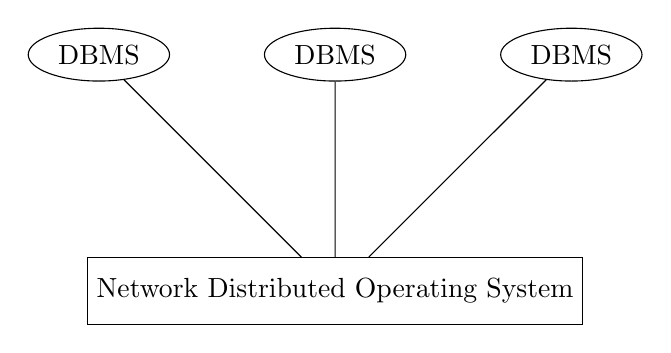
\begin{tikzpicture}[auto,node distance=5cm,level distance=3cm]

  \node[entity] (node1) {Network Distributed Operating System}
    [grow=up,sibling distance=3cm]
    child {node[attribute] {DBMS} }
    child {node[attribute] {DBMS}}
    child {node[attribute] {DBMS}};

\end{tikzpicture}


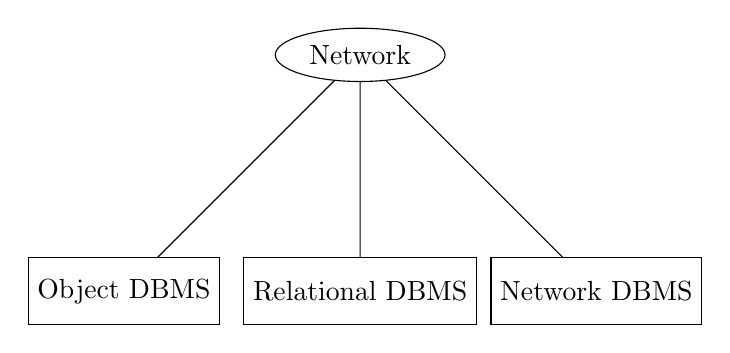
\begin{tikzpicture}[auto,node distance=5cm,level distance=3cm]

  \node[attribute] (node1) {Network}
    [grow=down,sibling distance=3cm]
    child {node[entity] {Object DBMS} }
    child {node[entity] {Relational DBMS}}
    child {node[entity] {Network DBMS}};

\end{tikzpicture}


\begin{tikzpicture}[auto]%,node distance=5cm,level distance=3cm]

  \node[entity] (node1) {دانشجو};

  \node[entity] (node2) [above right = of node1]	{استاد};
  \node[entity] (node3) [above left = of node1]	{دانشکده};
  \node[entity] (node4) [below right = of node1]	{درس};
  \node[entity] (node5) [below left = of node1]	{کلاس};
  % Draw an edge between rel1 and node1; rel1 and node2
  %\path (rel1) edge node {1-\(m\)} (node1)
  %  edge	 node {\(n\)-\(m\)}	(node2);

\end{tikzpicture}



\begin{tikzpicture}[auto]%,node distance=5cm,level distance=3cm]

  \node[entity] (node1) {دانشجو};

  \node[attribute] (node2) [above right = of node1]	{شماره-دانشجویی};
  \node[attribute] (node3) [above left = of node1]	{تولد};
  \node[attribute] (node4) [below right = of node1]	{نام};
  \node[attribute] (node5) [below left = of node1]	{آدرس};
  Draw an edge between node1 and node2; node1 and node3;
  node1 and node4; node1 and node5;
  
  \path (node1) edge node {} (node2)
    edge node {} (node3)
    edge node {} (node4)
    edge node {} (node5);

\end{tikzpicture}




\begin{tikzpicture}[node distance=6em]

  \node[entity] (emp) {Employee};
    \node[attribute] (e_id) [left=2em of emp] {} edge (emp);
    \node[attribute] (e_name) [right=2em of emp] {} edge (emp);
    \node[attribute] (e_sal) [above=2em of emp] {} edge (emp);

  \node[relationship] (works) [below of=emp, node distance=8em] {} edge (emp);

  \node[entity] (dept) [below of=works, node distance=8em] {} edge (works);
    \node[attribute] (d_num) [left=2em of dept] {} edge (dept);
    \node[attribute] (d_name) [right=2em of dept] {} edge (dept);

\end{tikzpicture}



\begin{tikzpicture}[node distance=6em]

  \node[entity] (emp) {فروش};
    \node[attribute] (e_id) [right=2em of emp] {فروشنده} edge (emp);
    \node[attribute] (e_name) [below=2em of emp] {مشتری} edge (emp);
    \node[attribute] (e_sal) [left=2em of emp] {محصول} edge (emp);

  %\node[relationship] (works) [below of=emp, node distance=8em] {} edge (emp);

  %\node[entity] (dept) [below of=works, node distance=8em] {} edge (works);
  %  \node[attribute] (d_num) [left=2em of dept] {} edge (dept);
  %  \node[attribute] (d_name) [right=2em of dept] {} edge (dept);

\end{tikzpicture}



\begin{tikzpicture}[node distance=6em]

  \node[entity] (emp) {فروش};
    \node[entity] (e_id) [right=2em of emp] {فروشنده} edge (emp);
    \node[entity] (e_name) [below=2em of emp] {مشتری} edge (emp);
    \node[entity] (e_sal) [left=2em of emp] {محصول} edge (emp);

  %\node[relationship] (works) [below of=emp, node distance=8em] {} edge (emp);

  %\node[entity] (dept) [below of=works, node distance=8em] {} edge (works);
  %  \node[attribute] (d_num) [left=2em of dept] {} edge (dept);
  %  \node[attribute] (d_name) [right=2em of dept] {} edge (dept);

\end{tikzpicture}






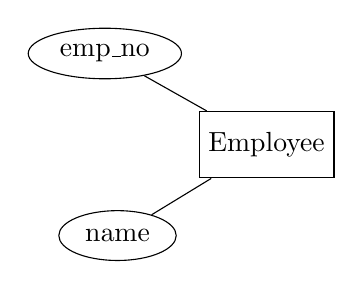
\begin{tikzpicture}[node distance=6em]

  \node[entity] (emp) {Employee};
    \node[attribute] (e_id) [above left=2em of emp] {emp\_no} edge (emp);
    \node[attribute] (e_name) [below left=2em of emp] {name} edge (emp);
    
  %\node[relationship] (works) [below of=emp, node distance=8em] {} edge (emp);

  %\node[entity] (dept) [below of=works, node distance=8em] {} edge (works);
  %  \node[attribute] (d_num) [left=2em of dept] {} edge (dept);
  %  \node[attribute] (d_name) [right=2em of dept] {} edge (dept);

\end{tikzpicture}





\end{document}